\documentclass[12pt,]{book}
\usepackage[]{tgpagella}
\usepackage{amssymb,amsmath}
\usepackage{ifxetex,ifluatex}
\usepackage{fixltx2e} % provides \textsubscript
\ifnum 0\ifxetex 1\fi\ifluatex 1\fi=0 % if pdftex
  \usepackage[T1]{fontenc}
  \usepackage[utf8]{inputenc}
\else % if luatex or xelatex
  \ifxetex
    \usepackage{mathspec}
  \else
    \usepackage{fontspec}
  \fi
  \defaultfontfeatures{Ligatures=TeX,Scale=MatchLowercase}
\fi
% use upquote if available, for straight quotes in verbatim environments
\IfFileExists{upquote.sty}{\usepackage{upquote}}{}
% use microtype if available
\IfFileExists{microtype.sty}{%
\usepackage{microtype}
\UseMicrotypeSet[protrusion]{basicmath} % disable protrusion for tt fonts
}{}
\usepackage[margin=1in]{geometry}
\usepackage{hyperref}
\hypersetup{unicode=true,
            pdftitle={The Formation of New Rebel Groups},
            pdfauthor={David Bowden},
            pdfborder={0 0 0},
            breaklinks=true}
\urlstyle{same}  % don't use monospace font for urls
\usepackage{longtable,booktabs}
\usepackage{graphicx,grffile}
\makeatletter
\def\maxwidth{\ifdim\Gin@nat@width>\linewidth\linewidth\else\Gin@nat@width\fi}
\def\maxheight{\ifdim\Gin@nat@height>\textheight\textheight\else\Gin@nat@height\fi}
\makeatother
% Scale images if necessary, so that they will not overflow the page
% margins by default, and it is still possible to overwrite the defaults
% using explicit options in \includegraphics[width, height, ...]{}
\setkeys{Gin}{width=\maxwidth,height=\maxheight,keepaspectratio}
\IfFileExists{parskip.sty}{%
\usepackage{parskip}
}{% else
\setlength{\parindent}{0pt}
\setlength{\parskip}{6pt plus 2pt minus 1pt}
}
\setlength{\emergencystretch}{3em}  % prevent overfull lines
\providecommand{\tightlist}{%
  \setlength{\itemsep}{0pt}\setlength{\parskip}{0pt}}
\setcounter{secnumdepth}{5}
% Redefines (sub)paragraphs to behave more like sections
\ifx\paragraph\undefined\else
\let\oldparagraph\paragraph
\renewcommand{\paragraph}[1]{\oldparagraph{#1}\mbox{}}
\fi
\ifx\subparagraph\undefined\else
\let\oldsubparagraph\subparagraph
\renewcommand{\subparagraph}[1]{\oldsubparagraph{#1}\mbox{}}
\fi

%%% Use protect on footnotes to avoid problems with footnotes in titles
\let\rmarkdownfootnote\footnote%
\def\footnote{\protect\rmarkdownfootnote}

%%% Change title format to be more compact
\usepackage{titling}

% Create subtitle command for use in maketitle
\newcommand{\subtitle}[1]{
  \posttitle{
    \begin{center}\large#1\end{center}
    }
}

\setlength{\droptitle}{-2em}
  \title{The Formation of New Rebel Groups}
  \pretitle{\vspace{\droptitle}\centering\huge}
  \posttitle{\par}
  \author{David Bowden}
  \preauthor{\centering\large\emph}
  \postauthor{\par}
  \predate{\centering\large\emph}
  \postdate{\par}
  \date{June 27, 2017}

\usepackage{setspace}

\usepackage{float}
\let\origtable\table
\let\endorigtable\endtable
\renewenvironment{table}[1][2] {
    \singlespacing
    \expandafter\origtable\expandafter[H]
} {
    \endorigtable
}

\frontmatter

\usepackage{amsthm}
\newtheorem{theorem}{Theorem}[chapter]
\newtheorem{lemma}{Lemma}[chapter]
\theoremstyle{definition}
\newtheorem{definition}{Definition}[chapter]
\newtheorem{corollary}{Corollary}[chapter]
\newtheorem{proposition}{Proposition}[chapter]
\theoremstyle{definition}
\newtheorem{example}{Example}[chapter]
\theoremstyle{remark}
\newtheorem*{remark}{Remark}
\begin{document}
\maketitle

\doublespacing

\mainmatter

\chapter{The Formation of New Rebel Groups}\label{entry}

This chapter builds on the individual-level findings from Chapter
\ref{survey-chapter} to explain one aggregate manifestation of
repression --- the formation of entirely new rebel groups. Specifically,
I am interested in cases where entirely new rebel groups join ongoing
civil wars. By new I simply mean a group that has not previously
participated in violence. Pre-existing non-violent organizations such as
religious organizations or political parties could constitute a new
rebel group so long as they have not used violence previously, as would
entirely new organizations that form during a conflict. I distinguish
this sort of group formation from the splintering of existing
organizations, as I expect the causal processes to be somewhat
different. While splintering is driven by individuals who have already
resorted to violence deciding to reorganize, group formation has the
additional requirement of mobilizing previously non-violent individuals.
To the best of my knowledge, no existing study directly addresses this
question.

I expect that repression should increase the probability that a new
rebel group will enter an ongoing conflict. As previously peaceful
individuals experience violence, the relative cost for them to join a
rebellion decreases. These individuals will not necessarily be inclined
to join an existing rebel group, however. If an individual has been
repressed, existing groups have in some sense failed to protect them.
Furthermore, repression should tend to induce greater levels of ethnic
identification. Repression is often targeting on the basis of ethnicity,
increasing the salience of such identities. Ethnic identification may
also have instrumental value in attracting support from outside
co-ethnic states, and repression may give these outside states both
motive and political cover for supporting new rebel groups. Thus, there
should be a relationship between repression and the emergence of new
rebel groups.

\emph{Hypothesis 3: The probability that a new rebel group will form
should increase with the level of repression in the country}

If ethnic polarization is the mechanism behind rebel group formation,
the ethnic diversity of a country should provide an important scope
condition. It would be unlikely for repression to induce ethnic
identification in a very homogeneous society, for instance. In such
cases a different social cleavage might be activated, or repression
might not sow division among dissidents at all. I thus expect a positive
interaction between repression and ethnic diversity, with repression
increasing the probability of new rebel groups at higher levels of
diversity, while being less effective at low levels of diversity.

\emph{Hypothesis 4: There should be a positive interaction between
repression and ethnic diversity}

My theory suggests that individuals form new rebel groups largely
because repression begins to polarize society on the dimension of ethnic
identity. This argument has a testable implication regarding the new
rebel groups that emerge --- they should be likelier than pre-existing
groups to draw their support from a single ethnic group.

\emph{Hypothesis 5: Rebel groups that join ongoing conflicts should be
more likely than others to draw their support from a single ethnic
group}

\section{Research Design}\label{research-design}

To test the preceding hypotheses I use a dataset of country war-years
derived from the Uppsala Conflict Data Program and Peace Research
Institute Oslo's Dyadic Dataset, version 4-2016 (Harbom, Melander, and
Wallensteen \protect\hyperlink{ref-Harbom2008}{2008}; Melander,
Pettersson, and Themnér \protect\hyperlink{ref-Melander2016}{2016}).
This dataset includes one observation for every government-rebel group
dyad for each year in which it produced at least 25 fatalities. I
exclude all interstate conflicts from the data, and include all civil
wars, anti-colonial wars, and internationalized civil wars. The
remaining rebel dyads are grouped into conflicts, with all rebels
seeking to overthrown the central government considered to be part of
the same conflict, and separatist movements grouped together if they are
pursuing independence for the same territory. Thus conflicts can contain
multiple rebel groups, and countries can contain multiple conflicts. I
then aggregate this data to the conflict-year, as my outcome of interest
is whether a new rebel group joined the fighting in a given year. This
results in a dataset of 2,048 observations, covering the period
1946--2015. The advantage of using conflict-years rather than
aggregating to country-years is that I am able to examine the effects of
several covariates measured at the conflict level, including conflict
intensity and the type of issue at stake. The use of conflict-years does
create a methodological challenge, however, as many of my covariates are
measured at the country level. To combat this I cluster the standard
errors by country. Additionally, aggregating the data to the
country-year does not substantially change the results.

\subsection{Dependent Variables}\label{dependent-variables}

\subsubsection*{Entry of New Rebel
Groups}\label{entry-of-new-rebel-groups}
\addcontentsline{toc}{subsubsection}{Entry of New Rebel Groups}

My primary dependent variable in this study is the entry of new rebel
groups to an ongoing conflict. To qualify, a rebel group must meet two
criteria. First, it cannot have previously participated in political
violence. To determine this I use rebel origins data I collected
(described in the Chapter 2 Appendix), and exclude groups that
originated as portions of different rebel groups --- splinter
organizations and alliances. This leaves rebel groups that emerged out
of non-violent organizations such as political organizations, as well as
militarized, but not political organizations such as local defense
militias. Second, the group must join an ongoing conflict. I define a
conflict as ongoing if it has produced at least 25 fatalities in at
least one of the past three years. If three consecutive years of peace
occur, I consider the next round of fighting to be a new conflict
episode, and any new rebel groups that appear in the first year of an
episode are considered to have initiated that conflict rather than
joined it.

Of the 503 rebel groups that appear in my data, 83 fit the definition.
As some of these entered the same conflict in the same year, 73 of
2045\footnote{Some observations are left-censored, meaning I am unable
  to determine whether there was conflict during the previous three
  years as it would predate the beginning of the dataset.} (5.6\%) of
conflict-years are coded as having a new rebel group.

\subsubsection*{Rebel Group Ethnicity}\label{rebel-group-ethnicity}
\addcontentsline{toc}{subsubsection}{Rebel Group Ethnicity}

\emph{H5} predicts that because the formation of new rebel groups is
driven by a broader reorganization of society along ethnic lines, these
newly-formed rebel groups should be likelier than others to draw their
support from a single ethnic group. To test this I use the ACD2EPR 2014
dataset (Wucherpfennig et al.
\protect\hyperlink{ref-Wucherpfennig2011}{2011}; Vogt et al.
\protect\hyperlink{ref-Vogt2015}{2015}), which links rebel groups from
the Uppsala Armed Conflict Data v.4-2014 (Melander, Pettersson, and
Themnér \protect\hyperlink{ref-Melander2016}{2016}) to ethnic groups
from the Ethnic Power Relations (EPR-Core 2014) (Cederman, Wimmer, and
Min \protect\hyperlink{ref-Cederman2010}{2010}; Vogt et al.
\protect\hyperlink{ref-Vogt2015}{2015}). This dataset identifies three
forms of linkages between ethnic groups and rebel groups. First, a rebel
group can claim to operate exclusively on behalf of a particular ethnic
group. The dataset does allow for the possibility that a group could
make such claims for multiple ethnic groups, as was the case for several
of the South Sudanese separatist groups. Second, the data records all of
the ethnic groups from which a rebel group recruits a significant number
of soldiers. Finally, the data codes whether at least 50\% of the
members of an ethnic group support a rebel group. I collapse these
measures into a single count of the number of ethnic groups to which a
rebel group is tied. I then categorize rebel groups as ``mono-ethnic,''
``multi-ethnic,'' or ``non-ethnic,'' if they have no such ties. The
distribution of cases across these categories is reported in Table
\ref{tab:acd2epr}.

\begin{longtable}[]{@{}lll@{}}
\caption{\label{tab:acd2epr} Rebel Groups by Ethnic
Affiliation}\tabularnewline
\toprule
Non-Ethnic & Mono-Ethnic & Multi-Ethnic\tabularnewline
\midrule
\endfirsthead
\toprule
Non-Ethnic & Mono-Ethnic & Multi-Ethnic\tabularnewline
\midrule
\endhead
97 & 309 & 47\tabularnewline
\bottomrule
\end{longtable}

\subsection{Independent Variables}\label{independent-variables}

\subsubsection*{Human Rights}\label{human-rights}
\addcontentsline{toc}{subsubsection}{Human Rights}

To measure repression I use the same country-level measure employed in
Chapter \ref{survey-chapter}, the Latent Human Protection scores,
version 2 (Fariss \protect\hyperlink{ref-Fariss2014}{2014}; Schnakenberg
and Fariss \protect\hyperlink{ref-Schnakenberg2014}{2014}). The
motivation for this data project is the fact that human rights measures
are typically based on media reports, creating the possibility that both
the depth of coverage and standards against which human rights practices
are evaluated might vary across space and time. To solve this, the
dataset uses thirteen data sources including U.S. State Department and
Human Rights Watch reports and most major scholarly datasets in a
Bayesian measurement model. This produces an estimate for each
country-year based on a mix of the data for that particular year and the
average score for that country and year. While this creates a human
rights measure that is comparable across contexts, one disadvantage is
that the units are not inherently meaningful, only providing a basis for
comparison across observations.

The measure ranges from roughly -3.1 (most repressive) to 4.7 (most
respectful of human rights). The average score across the full sample of
post-World War II country-years is 0.29, while in my sample of countries
experiencing civil war the mean is -1.24, with a range from -3.11 to
1.51. Thus, the sample includes the full range of repressive states,
while unsurprisingly lacking any states with especially strong human
rights practices. For reference, recent country-years with scores around
1.5 including Hungary in 2011, and France in 2007. In other words, these
are typically cases in which citizens are generally safe from physical
harm, but some minorities such as Muslims in France experience political
and economic discrimination. Russia in recent years falls in the middle
of the spectrum, with scores around 1.0. Examples of cases towards the
more repressive end of the spectrum include Saddam Hussein's Iraq, which
had a score averaging around -2.5, and Sudan, which had scores around
-3.0 during the genocide in Darfur.

The raw Latent Human Protection Scores tend to be relatively static over
time. Yet, my theory suggests that it is changes in human rights
practices, in the direction of being more repressive, that should change
dissident behavior. To ensure that I am capturing these pheonemena, I
use the year-over-year change in human protection score. While the
average conflict-year sees very little change from the preceding year
(the mean change is -0.01), 110 cases experience a negative change of at
least 0.25, and in one case the score decreased by 2.52 in a single
year. I lag the measure by one year, meaning that I am ultimately using
the change in human rights practices at time \emph{t} to predict the
formation of new rebel groups at time \emph{t+1}.

\subsubsection*{Ethnic Diversity}\label{ethnic-diversity}
\addcontentsline{toc}{subsubsection}{Ethnic Diversity}

\emph{H4} suggests that ethnic diversity should place a scope condition
on my theory, with the formation of new groups being less likely at very
high and low levels of ethnic diversity. I first test for the effect of
ethnic diversity individually by including the raw and squared
ethnolinguistic fractionalization as predictors. This tests for a
curvilinear relationship, allowing for the effect of the variable to
differ at moderate and extreme values. The data come from Fearon and
Laitin (\protect\hyperlink{ref-fearonlaitin03}{2003}), and can be
interpreted as the probability that two individuals drawn at random will
be able to communicate. In addition to testing whether ethnic diversity
affects the probability of new group formation on its own, I also test
whether it alters the performance of the human rights measure, by
interacting the latter with both the raw and squared ethnolinguistic
fractionalization measures.

\subsubsection*{New Rebel Group Entry}\label{new-rebel-group-entry}
\addcontentsline{toc}{subsubsection}{New Rebel Group Entry}

\emph{H5} predicts that the rebel groups that form during ongoing
conflicts should be more likely than others to be tied to a single
ethnic group. Thus the new rebel group entry variable becomes an
independent variable in this analysis, predicting the ethnic composition
of rebel groups.

\subsection{Control Variables}\label{control-variables}

I control for several factors that might confound my results. To account
for the possibility that human rights scores are simply a function of
conflict intensity, rather than discriminatory intent, I include the
maximum conflict intensity value from the UCDP Dyadic data. The measure
is binary, with a value of 1 indicating that the dyad produced between
25 and 999 fatalities in a given year, and a value of 2 indicating that
the dyad produced 1,000 or more fatalities. This measure is moderately
correlated with the human rights score (Pearson's r = -0.30). The exact
measure of fatalities available for the post-1989 period is even less
correlated (Pearson's r = -0.25). Thus, human rights practices are for
the most part measuring something distinct from conflict intensity.

Conflicts that already have multiple rebel groups may have some
unobserved quality that makes them more likely to have fragmented rebel
movements. For example, there might be a history of personal animosity
between rebel elites (see Christia
\protect\hyperlink{ref-Christia2012}{2012}). To capture such effects, I
include a binary indicator of whether a conflict had multiple rebel
groups in the previous year.

Two standard controls from past conflict studies are also likely to be
relevant. One potential mechanism that might produce increased numbers
of rebel groups in a conflict is the movement of groups from a
neighboring civil war into a new conflict. To control for this
possibility I construct an indicator for the presence of a civil war in
a state that is contiguous by land using the UCDP Dyadic data and the
Correlates of War Direct Contiguity data, version 3.2 (Stinnett et al.
\protect\hyperlink{ref-Stinnett2002a}{2002}). As secessionist movements
are often (though not always) tied to a specific ethnic group, my
hypothesized theoretical mechanism should be less likely to apply in
such conflicts. Thus, I include a binary indicator of whether a conflict
is secessionist as opposed to being fought over control of the central
government.

I also control for several country-level factors. Conceivably, the
number of rebel groups in a country might simply be a function of the
country's size. I thus include a measure of the countries area in logged
square kilometers from the World Bank (The World Bank
\protect\hyperlink{ref-WorldBank2015}{2015}), and logged population and
logged GDP per capita from Gleditsch
(\protect\hyperlink{ref-Gleditsch2002b}{2002}). The characteristics of a
country's terrain might also matter, with mountainous areas both
creating more opportunities for rebellion, and more challenges in
coordinating rebel activities across space. To control for this affect I
include Fearon and Laitin's (2003) measure of the percentage of a
country's terrain that is mountainous. As democratic competition might
provide another incentive for ethnic identification (Eifert, Miguel, and
Posner \protect\hyperlink{ref-Eifert2010}{2010}), I include the
country's Polity IV regime score (Marshall, Gurr, and Jaggers
\protect\hyperlink{ref-Marshall2016}{2016}). The international context
could conceivably play an important role in rebel group formation, for
instance by shaping the availability of external support. I thus include
a binary indicator of whether a country-year occurred during or after
the Cold War.

Finally, the presence of natural resources may influence the functioning
of my theoretical mechanism. My theory assumes that rebel elites desire
the support of dissident constituents. If rebel groups are able to
procure sufficient funds and war materiel through the sale of natural
resources, however, they might care little about civilians (see
Weinstein \protect\hyperlink{ref-Weinstein2007}{2007}). I thus include a
count of the number of locations in a country containing `lootable'
natural resources, meaning those which can be extracted with relatively
unsophisticated operations. The resources included in the measure are
oil (Lujala, Rød, and Thieme \protect\hyperlink{ref-Lujala2007}{2007}),
diamonds (Gilmore et al. \protect\hyperlink{ref-Gilmore2007}{2005};
Lujala, Gleditsch, and Gilmore
\protect\hyperlink{ref-Lujala2005}{2005}), gold (Balestri
\protect\hyperlink{ref-Balestri2012}{2012}), gems (Lujala
\protect\hyperlink{ref-Lujala2008}{2008}), and drugs (Buhaug and Lujala
\protect\hyperlink{ref-Buhaug2005}{2005}).

\subsection{Statistical Model}\label{statistical-model}

As the dependent variable in this study is a binary measure of whether a
new rebel group entered a conflict in a given year, I use a logistic
regression model. For robustness, I examine several variants of the
model. These include a model with fixed effects for country and year,
and a rare-events correction to account for the fact that group
formation occurs in only a small portion of my cases. I also cluster the
standard errors by country, as many of my variables are measured at the
country-level, creating the possibility that errors could be correlated
across different conflicts in the same country. I also estimate models
(not reported) with the country-year as the unit of analysis. None of
these changes substantially alters the results for my variables of
interest.

\section{Results}\label{results}

\subsection{Group Formation Results}\label{group-formation-results}

The logistic regression results are reported in Table \ref{tab:entry}.
Model 1 includes only the change in human rights measure, Model 2 adds a
battery of controls, Model 3 includes an interaction effect between
human rights and ethnolinguistic fractionalization, and Model 4 replaces
the (mostly) static country-level variables with fixed effects for
conflict and year.

In the three models without interaction terms the Change in Human Rights
variable performs as I expect. It is consistently negatively related to
the probability of new rebel group formation. The relationship is
statistically significant at the 99\% level in all three models. The
substantive effect is large, with a one-unit (which equates to roughly
1.5 standard deviations) decrease in human rights practices being
associated with a roughly 400\% increase in the odds of new rebel group
formation. While the predicted probability of a new rebel group emerging
is quite low when the change in human rights practices is zero (around
0.03, see Figure \ref{fig:effectplot}), at the largest decreases (a
change of -2.5 in one year) the probability of a new rebel group
emerging is 0.72. The effect size is similar across models. With these
results I am able to reject the null hypothesis of no relationship
between repression and the formation of new rebel groups, consistent
with my expectation in \emph{Hypothesis 4}.

\begin{table}
\begin{center}
\begin{tabular}{l c c c c }
\hline
 & Model 1 & Model 2 & Model 3 & Model 4 \\
\hline
(Intercept)                             & $-3.27^{***}$ & $6.69^{*}$   & $7.00^{*}$ & $15.71$      \\
                                        & $(0.13)$      & $(3.03)$     & $(3.13)$   & $(14503.27)$ \\
Change in Human Rights                  & $-1.37^{***}$ & $-1.41^{**}$ & $-1.53$    & $-1.79^{**}$ \\
                                        & $(0.33)$      & $(0.43)$     & $(2.11)$   & $(0.59)$     \\
Ethnolinguistic Fractionalization       &               & $-5.78$      & $-5.95$    &              \\
                                        &               & $(3.16)$     & $(3.30)$   &              \\
Ethnolinguistic Fractionalization$^{2}$ &               & $6.24$       & $6.65^{*}$ &              \\
                                        &               & $(3.21)$     & $(3.31)$   &              \\
Human Rights X Fractionalization        &               &              & $-6.44$    &              \\
                                        &               &              & $(9.86)$   &              \\
Human Rights X Fractionalization$^{2}$  &               &              & $9.91$     &              \\
                                        &               &              & $(10.10)$  &              \\
Intensity Level                         &               & $-0.19$      & $-0.22$    & $-0.23$      \\
                                        &               & $(0.39)$     & $(0.40)$   & $(0.44)$     \\
Prev. Multi-rebel                       &               & $0.16$       & $0.16$     & $-0.95^{**}$ \\
                                        &               & $(0.39)$     & $(0.39)$   & $(0.36)$     \\
Contiguous Civil War                    &               & $-0.05$      & $-0.05$    & $0.29^{*}$   \\
                                        &               & $(0.11)$     & $(0.11)$   & $(0.14)$     \\
Secessionist                            &               & $-1.00^{*}$  & $-0.91$    &              \\
                                        &               & $(0.47)$     & $(0.47)$   &              \\
Logged Area                             &               & $-0.18$      & $-0.17$    &              \\
                                        &               & $(0.18)$     & $(0.18)$   &              \\
Mountainous Terrain                     &               & $0.00$       & $0.01$     &              \\
                                        &               & $(0.01)$     & $(0.01)$   &              \\
Logged GDP per capita                   &               & $-0.33$      & $-0.36$    &              \\
                                        &               & $(0.25)$     & $(0.25)$   &              \\
Logged Population                       &               & $-0.37$      & $-0.42$    &              \\
                                        &               & $(0.25)$     & $(0.25)$   &              \\
Polity                                  &               & $-0.01$      & $-0.00$    &              \\
                                        &               & $(0.03)$     & $(0.03)$   &              \\
Post Cold War                           &               & $-0.25$      & $-0.18$    &              \\
                                        &               & $(0.38)$     & $(0.39)$   &              \\
Lootable Resource Sites                 &               & $-0.00$      & $-0.00$    &              \\
                                        &               & $(0.01)$     & $(0.01)$   &              \\
\hline
AIC                                     & 521.11        & 317.57       & 318.26     & 585.79       \\
BIC                                     & 531.86        & 392.19       & 402.83     & 1263.99      \\
Log Likelihood                          & -258.55       & -143.78      & -142.13    & -164.90      \\
Deviance                                & 517.11        & 287.57       & 284.26     & 329.79       \\
Num. obs.                               & 1597          & 1069         & 1069       & 1478         \\
\hline
\multicolumn{5}{l}{\scriptsize{$^{***}p<0.001$, $^{**}p<0.01$, $^*p<0.05$}}
\end{tabular}
\caption{Logit Models of Rebel Group Formation}
\label{tab:entry}
\end{center}
\end{table}

Model 3 provides a test of the interaction proposed in \emph{H5}.
Whereas I expect an interaction effect between the human rights measure
and ethnolinguistic fractionalization, the two coefficents testing this
(there are two as I expect the effect of ethnolinguistic
fractionalization to be curvilinear) are not statistically significant.
Ethnic diversity does not seem to matter on its own, either, as there is
no evidence of a curvilinear effect, nor of a linear effect (not
reported). I am thus unable to reject the null hypothesis of no
relationship between ethnic diversity and the probability of new rebel
groups forming. It is unclear whether this means my hypothesized
mechanism of increased ethnic salience operates even at extreme levels
of diversity, or if other mechanisms might operate in those cases. The
analysis later in this chapter sheds light on that question.

\begin{figure}
\centering
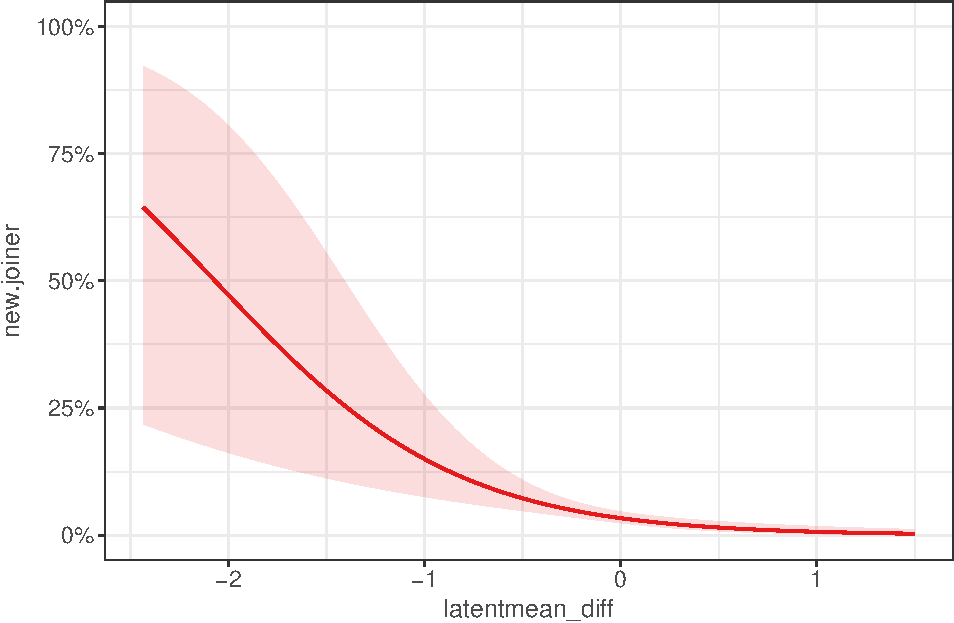
\includegraphics{entry_standalone_files/figure-latex/effectplot-1.pdf}
\caption{\label{fig:effectplot}Predicted Probability of New Rebel Group
Formation (Based on Model 2)}
\end{figure}

Only a few control variables are significant, likely reflecting the fact
that rebel group formation is a rare and time-varying outcome, while
many of the predictors are largely static. New rebel groups are less
likely in secessionist conflicts. As these conflicts are often fought by
an ethnically homogeneous movement, this result is consistent with my
overarching belief that the formation of new groups is about fighting on
behalf of previously underrepresented ethnic groups. The `Previously
Multi-Rebel' measure is negatively related the probability of further
groups joining, though only in the fixed effects model. This result
perhaps suggests that rather than portending further fragmentation of
the rebel movement, the presence of multiple rebel groups might signal
that a conflict has become saturated with factions, and further
additions are unlikely. Contiguous civil wars have a significant
positive relationship, suggesting that some new rebel groups might be
transnational in character. Again, however, the result is only
significant in the fixed effects model.

These results are robust to a number of manipulations. The raw Latent
Human Protection Score also consistently predicts the formation of new
groups, though the substantive effect is slightly smaller than that of
the differenced measure I employ. As mentioned, the results are similar
when the data are aggregated into conflict years rather than treating
separatist movements as distinct conflicts. I also include attributes of
the largest rebel group active in the previous year, such as its size,
degree of centralization, and whether it received foreign support. None
change the performance of my human rights measure.

I do not perform any sort of causal identification in this analysis. I
have examined several measures of oil production as potential
instruments for repression, but none came close to the conventional
standard for a strong instrument.\footnote{An instrument is considered
  strong if the first-stage F-statistic is at least 10 (Angrist and
  Pischke \protect\hyperlink{ref-Angrist2009}{2009}). The scores for the
  oil measures were generally around 4.5.} Matching is not an ideal
choice here, as it requires a binary treatment, and my human rights
measure is continuous. I cannot rule out the possibility that my results
actually reflect the government's ability to anticipate new rebellions.
Given that a rebel group must produce 25 fatalities in a calendar year
before it enters the data, it is possible for an organization to exist,
and for the government to be aware of it, in the years prior to it being
coded as a new group in my data. However, I am skeptical that the
temporal structure of such a process would be consistent enough to
produce the results I report here --- it is unlikely that the increase
in repression would consistent occur one year before the rebel group
produces 25 fatalities, rather two or three years prior.

Ultimately, these results provide strong support for \emph{H4}, as
changes in human rights are robustly related to the formation of new
rebel groups. I do not find support that ethnic diversity is related to
this outcome, as I predicted in \emph{H5}. Yet, this hypothesis is
intended to establish scope conditions. The lack of support could then
be an indication that my theory applies more broadly than I expected.

\subsection{Group Composition Results}\label{group-composition-results}

\emph{H6} predicts that the groups which join ongoing conflicts should
be more likely than others to draw their support from a single ethnic
group. This proposition is tested in Table \ref{tab:comp}. These
analyses use the rebel group as the unit of analysis, with the ethnic
composition of the group being the dependent variable. In Model 5 the
dependent variable is monoethnic composition, in Model 6 it is
multiethnic composition, and in Model 7 it is nonethnic composition,
meaning the group has no discernible ties to a politically-relevant
ethnic group. I include two group-level covariates from the Non-State
Actor Dataset (Cunningham, Gleditsch, and Salehyan
\protect\hyperlink{ref-Cunningham2009}{2009}): binary indicators of
whether the group was active in a previous conflict, and whether it is a
transnational organization.

\begin{table}
\begin{center}
\begin{tabular}{l c c c }
\hline
 & M5 Monoethnic & M6 Multiethnic & M7 Nonethnic \\
\hline
(Intercept)                      & $0.22$       & $-3.67^{***}$ & $-0.11$     \\
                                 & $(0.29)$     & $(0.63)$      & $(0.30)$    \\
Joiner                           & $0.69^{*}$   & $-1.13$       & $-0.37$     \\
                                 & $(0.34)$     & $(0.65)$      & $(0.37)$    \\
Secessionist                     & $1.10^{***}$ & $-1.10^{*}$   & $-0.82^{*}$ \\
                                 & $(0.30)$     & $(0.49)$      & $(0.36)$    \\
Previously Active                & $0.10$       & $0.34$        & $-0.37$     \\
                                 & $(0.36)$     & $(0.49)$      & $(0.46)$    \\
Ethnlinguistic Fractionalization & $0.20$       & $2.10^{*}$    & $-1.18^{*}$ \\
                                 & $(0.45)$     & $(0.85)$      & $(0.51)$    \\
Transnational                    & $0.08$       & $1.06^{*}$    & $-0.71^{*}$ \\
                                 & $(0.26)$     & $(0.41)$      & $(0.31)$    \\
\hline
AIC                              & 393.55       & 193.44        & 323.48      \\
BIC                              & 416.22       & 216.11        & 346.14      \\
Log Likelihood                   & -190.78      & -90.72        & -155.74     \\
Deviance                         & 381.55       & 181.44        & 311.48      \\
Num. obs.                        & 323          & 323           & 323         \\
\hline
\multicolumn{4}{l}{\scriptsize{$^{***}p<0.001$, $^{**}p<0.01$, $^*p<0.05$}}
\end{tabular}
\caption{Logit Models of Rebel Group Ethnic Composition}
\label{tab:comp}
\end{center}
\end{table}

Consistent with \emph{H6}, I find that rebel groups that join ongoing
conflicts are nearly twice as likely as others to be monoethnic. The
relationship is statistically significant at the 95\% level. Joining
status is not related to multiethnic or nonethnic composition.
Secessionist groups are also more likely than others to be monoethnic,
while being significantly less likely to be multiethnic or nonethnic.
Unsurprisingly, the level of ethnolinguistic fractionalization in a
country is positively related to the probability that rebel groups there
will be multiethnic, and negatively related to their likelihood of being
nonethnic. Finally transnational groups are more likely than others to
be multiethnic, and less likely to lack an ethnic affiliation.

This analysis provides support both for \emph{Hypothesis 6}, and for my
broader theoretical framework. I expect that the entry of new rebel
groups to ongoing conflicts is the manifestation of increased
mobilization around ethnic identity. The fact that rebel groups of this
kind are significantly more likely than others to draw their support
from a single ethnic group provides strong evidence for this argument.
Future work should delve deeper into group attributes, looking not only
at recruitment and claims of representation, but also the platform that
rebel groups adopt. I would expect that joining groups would tend to
place greater emphasis on ethnic grievances than others.

\section{Burma Case Study}\label{burma-case-study}

To provide a more detailed examination of the processes leading to the
formation of new rebel groups, I conduct a qualitative case study of
Burma.\footnote{The country's military regime began using the name
  ``Myanmar'' in 1989, but most dissidents and the U.S. government
  continue to use ``Burma.''} Burma is in many respects among the most
ethnically-polarized societies in the world, as it has 11 separatist
movements. I argue that some of these movements have followed a pattern
of rebel organization that tracks closely with my theory. One advantage
of choosing this case is that potentially confounding factors such as
the presence of natural resources and support from outside states varies
substantially across separatist movements, while holding many other
factors constant including government attributes and colonial history.
Burma is also home to several rebel groups that do not conform perfectly
to my theoretical framework, providing an opportunity to refine my
explanation and identify scope conditions.

\begin{figure}

{\centering 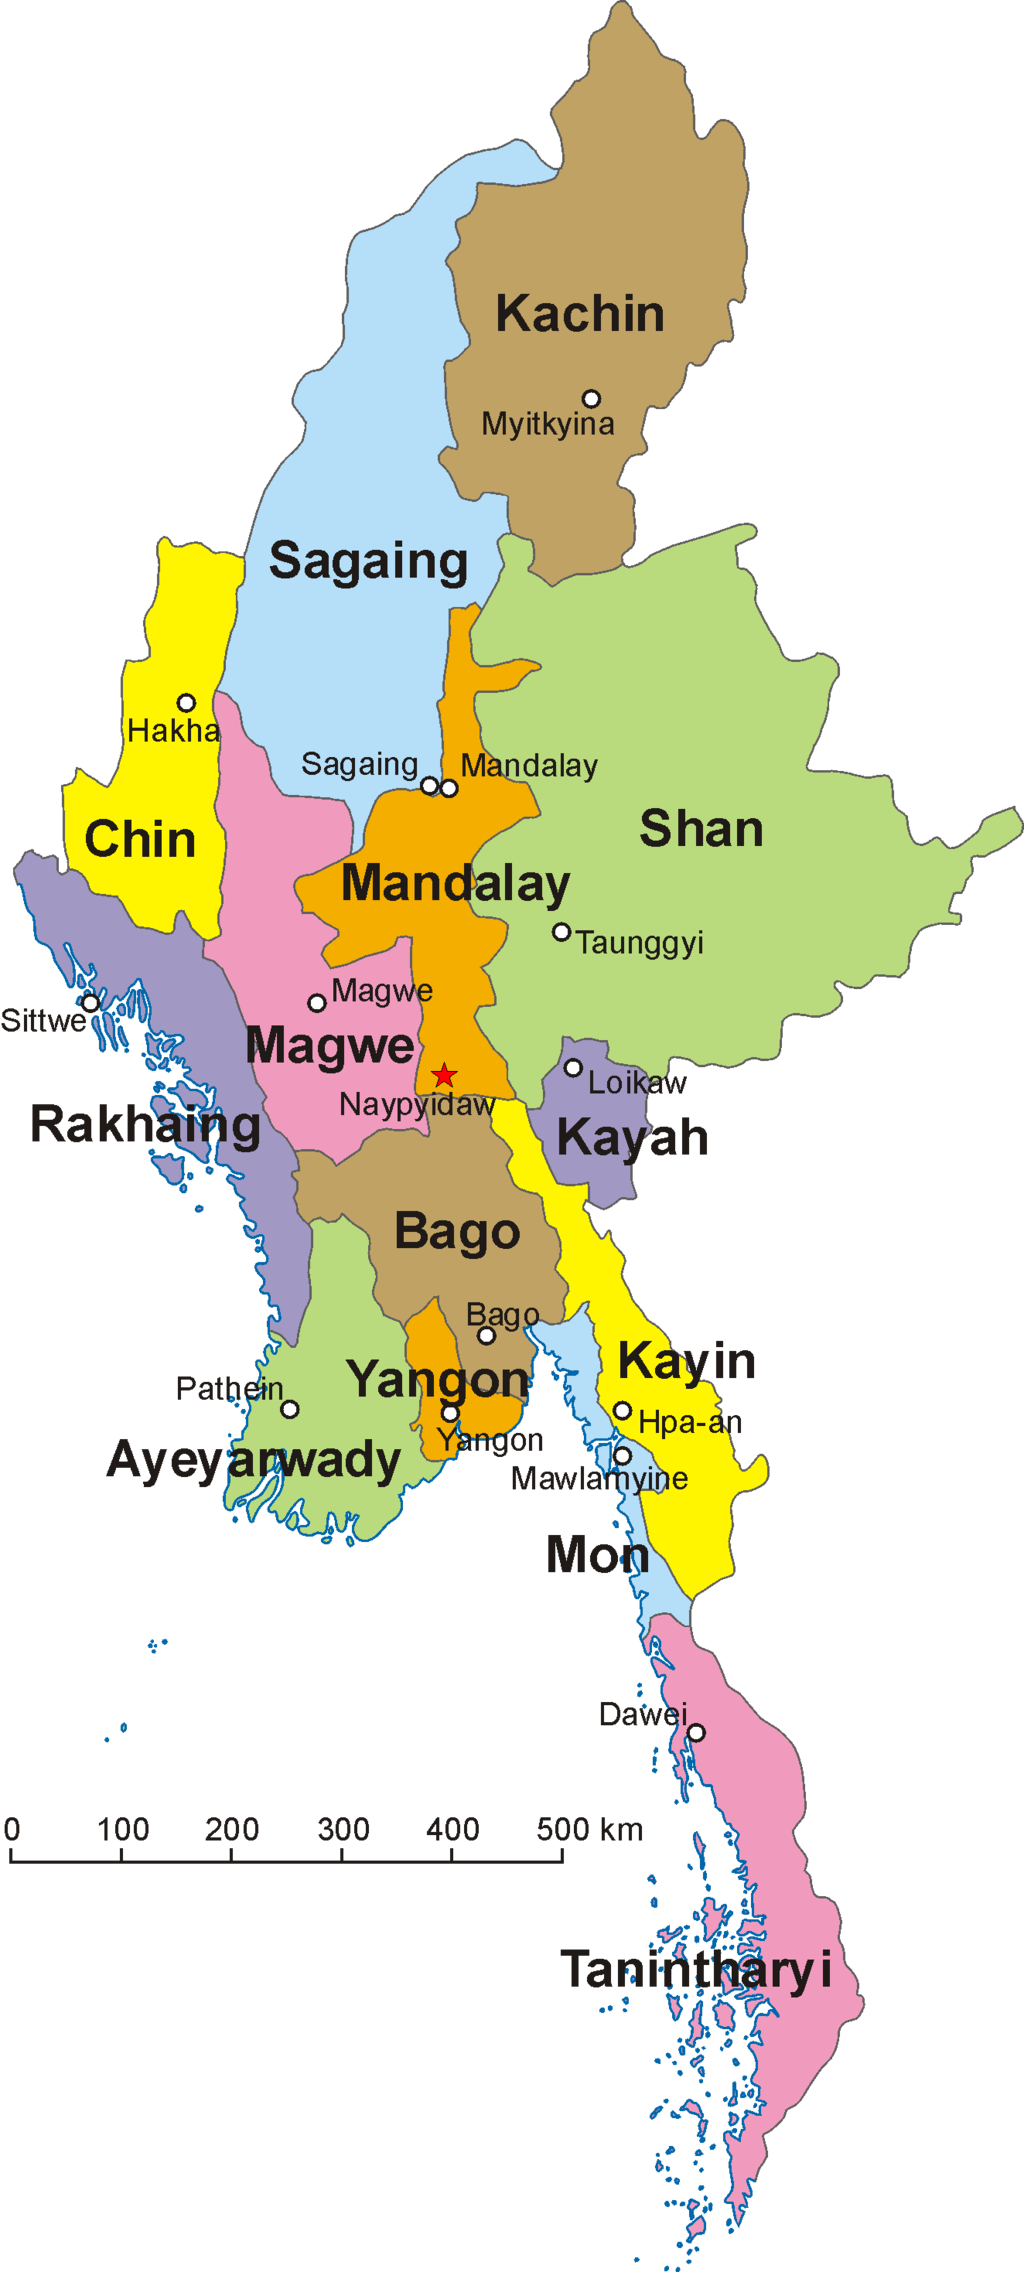
\includegraphics[width=0.5\linewidth]{~/Dropbox/Dissertation/Document/entry_chapter/Burma_en} 

}

\caption{Administrative Districts of Burma. Source: Aotearoa.}\label{fig:burmamap}
\end{figure}

As a whole, Burma is an ethnically diverse society, though ethnic
minorities tend to be concentrated on the largely mountainous periphery
of the country, while ethnic Burmans predominate in the central lowlands
(Steinberg \protect\hyperlink{ref-Steinberg2010}{2010}). In the
pre-colonial era these ethnic identities were relatively fluid, both in
terms of their content and their membership (South
\protect\hyperlink{ref-South2008}{2008}). British colonial rule from
1885--1948 led ethnic categories to become both more calcified and more
salient, as they practiced direct rule over the ethnic Burmans in the
lowlands, while delegating significant autonomy to the ethnic minorities
of the mountainous regions (South
\protect\hyperlink{ref-South2008}{2008}). Furthermore, administrative
practices such as frequent censuses required individuals to declare
their ethnicity (Charney \protect\hyperlink{ref-Charney2009}{2009}), and
most positions in the colonial bureaucracy and security forces were
given to minorities, as the majority Burmans were viewed as a greater
threat to colonial rule (Steinberg
\protect\hyperlink{ref-Steinberg2010}{2010}). Japan occupied Burma
through much of World War II, further entrenching ethnic divisions as
the Burman majority collaborated with the Japanese, while many ethnic
minorities including the Karen and Kachin supported the Allies
(Steinberg \protect\hyperlink{ref-Steinberg2010}{2010}).

Late in the war the most prominent faction of pro-Japanese Burmans, led
by Aung San, switched sides to support Allied efforts to liberate the
country. Most of the politically-active population of Burma, including
most ethnic minorities, joined together to form the Anti-Fascist
People's Freedom League (AFPFL). The organization remained mostly
cohesive for several years after the war in pursuit of independence
(Charney \protect\hyperlink{ref-Charney2009}{2009}). As soon as Aung San
succeeded in negotiating a peaceful conferral of independence from the
British in January 1947, however, ethnic tensions re-emerged. The
Panglong Agreement the following month established the boundaries of the
new Burmese state, placing the minority-dominated Frontier Areas under
Burman control. As several of the minority groups, including the Karen,
had received tacit promises from the British that they would receive
independence as separate states, turmoil ensued (Steinberg
\protect\hyperlink{ref-Steinberg2010}{2010}). Almost immediately upon
gaining independence in 1948, Burma faced two civil wars --- a
secessionist campaign led by the Karen National Union, and a bid to
overthrow the central government by the Red Flag faction of the
Communist Party of Burma.

\subsection{The Arakanese Buddhist
Rebels}\label{the-arakanese-buddhist-rebels}

The Arakan state is located in Western Burma, along its border with
Bangladesh. Today the district is more commonly known as Rakhine state
(or Rakhaing in Figure \ref{fig:burmamap}), and is notable for being the
location of the humanitarian crisis centering around the forced
migration of the Rohingya people. In this case study I will relax the
assumption that different issues of contention constitute entirely
separate conflicts. While the country ultimately saw separatist
movements associated with 11 different territories, the dissident elites
who led these movements were mostly united within the AFPFL prior to
independence. In some cases rebels from different separatist regions
collaborated, even while pursuing different goals (Smith
\protect\hyperlink{ref-Smith1999}{1999}). Furthermore, in some cases
smaller ethnic groups initially participated in the movements of larger
ethnicities, before launching their own rebellion. For example the
Karenni originally participated in the separatist movement of their
relatives the Karen, before later launching their own rebellion (Uppsala
Conflict Data Program \protect\hyperlink{ref-UCDPEncyclopedia}{2016}).
In some cases, then, it might be more accurate to view the new
separatist movements in Burma as having joined a larger ongoing
conflict, rather than initiating an entirely new one. Under this
conception, even the first Arakan separatist groups, the Arakan People's
Liberation Party (APLP) and the Mujahid Party, would be considered as
joining an ongoing conflict in 1948. Even when applying the coding rules
of the quantitative analysis and treating these groups as initiating a
new conflict, two other Buddhist groups clearly qualifier as new groups
--- the Arakan National Liberation Party (ANLP) in 1964, and the Arakan
Liberation Party in 1977.

While Arakan is considered an ethnicity largely because it has a long
history as a unified polity, its residents are divided along religious
lines. Indeed, even in its earliest days (beginning in 1948) the
secessionist movement there was divided into a Muslim faction (the
Mujahid Party) and a Buddhist one (the APLP) (Fredholm
\protect\hyperlink{ref-Fredholm1993}{1993}). This illustrates an
important limitation of my theoretical and empirical approach. I focus
on ethnicity as I expect that it will be the most salient social
cleavage in most countries, because its importance in the context of
civil war has been well-established (see Cederman, Wimmer, and Min
\protect\hyperlink{ref-Cederman2010}{2010}), and because ethnicity is
more easily measured than most other dimensions of identity. Clearly,
however, other cleavages can take priority in some cases, and can
sub-divide ethnicity as is the case in Arakan. Thus, even though both
factions of Arakan residents share a common purpose of securing
independence from Burma, they adopt the potentially counterproductive
arrangement of being organized into separate rebel groups on the basis
of religion.

Ultimately, however, I view the Arakan separatist movement as largely
consistent with my theory. While I expect that repression will
ultimately lead ethnic groups to produce cohesive rebel groups organized
around their identity, and this stops short of occurring in Arakan due
to religious divisions, the reasons why Arakanese organize as they do
are largely consistent with my theory. I expect that individuals will
turn to ethnicity in the face of repression because 1) repression is
often targeted on the basis of ethnicity, increasing the salience of
such groupings, and 2) ethnicity often provides a useful basis for
defense from repression, as ethnic groups often have militias, and may
be able to attract support from co-ethnic outside states.

While Burma was nominally democratic from independence in 1948 until a
military coup in 1962, the quality of human rights in the country was
low. The Latent Human Protection Score for the country was around -1.47
during this period, making it a relatively repressive regime as the
global average over the period was 0.03. For comparison, the score
changed little after what is generally considered to be a very
repressive military regime took power. Thus, at the dawn of the Arakan
independence movement the Burmese government employed a level of
repression that I would expect to provoke increases in the number of
individuals resorting to violence, and to levels of ethnic
identification. But whereas I suspect that repression is generally
targeted disproportionately at certain ethnic groups, in Arakan the
targeting was more specific, with Muslims being disproportionately
targeted relative to Buddhists. In fact, the government renamed the
state ``Rakhine,'' a name that previously referred only to the Buddhist
subset, to emphasize their stance against the Muslim minority known as
the Rohingyas (Fredholm \protect\hyperlink{ref-Fredholm1993}{1993}). The
Burmese government has maintained a military deployment to the region
through much of the conflict, and while it has applied significant
repression to both religions, it has been especially brutal toward the
Rohingya, ultimately seeking to force the minority to migrate into
Bangladesh (Steinberg \protect\hyperlink{ref-Steinberg2010}{2010}).
Thus, the underlying logic of my theory would imply that as repression
is applied with respect to both ethnicity and religion, both dimensions
of identity should be salient.

Once deciding to rebel, it would not be a foregone conclusion that an
Arakense dissident would choose to form a new rebel group. The Communist
Party of Burma had a strong following in Arakan; joining the Red Flag
faction, or later the Communist Party of Arakan, might have been a
viable option for many. The Karen National Union was also active prior
to any significant military mobilization in Arakan. It is not obvious,
\emph{a priori}, why the various separatists would not band together, as
individually none could pose a serious threat to the Burmese government.
Indeed, most of the separatist movements agreed to ceasefires in the
1990's and 2000's without winning any concessions, or coming at all
close to military victory. Later in the conflict there were in fact
attempts to build multi-ethnic alliances (Smith
\protect\hyperlink{ref-Smith1999}{1999}). Initially, however, dissidents
generally choose to organize on the basis of ethnicity, in some cases
further subdivided by religion. Geographic isolation surely played some
role in the lack of coordination across regions, but in several cases
separatists operated outside of their own secessionist territory, and
Communist forces frequently traveled between different separatist
regions (Smith \protect\hyperlink{ref-Smith1999}{1999}). Furthermore,
the Arakanese and Karen separatists had been unified under the banner of
the AFLFP just a few months prior, meaning that at least at the elite
level, they had communication channels and a history of interaction. As
Staniland (\protect\hyperlink{ref-Staniland2014}{2014}) notes, social
groups with these sorts of ties are often able to build national rebel
groups. The fact that this did not occur suggests that ethnicity was an
important factor in preventing the consolidation of dissent.

After accounting for the religious cleavage, the organization of
Arakanese rebels is consistent with my expectations. Buddhists and
Muslims generally consolidated into a single rebel group each.
Interestingly, the specific organizations changed over time, with one
group being defeated and another taking its place. For example, when the
Arakan conflict began in 1948, Buddhists were represented by the Arakan
People's Liberation Party. The APLP was defeated in the late 1950's.
Surviving members joined with new recruits to form the Arakan National
Liberation Party a few years later. The ANLP too was defeated, only to
be later replaced by the Arakan Liberation Party. Thus while three new
Buddhist organizations joined the ongoing conflict in Arakan, they
seemingly replaced one another, and represented the same underlying
constituency. This suggests that dissidents only form new organizations
if there is not already a group representing their particular set of
identities. Furthermore, it suggests that there is a persistent demand
for rebel groups to provide representation. If an existing rebel group
is defeated, the potential support of dissident constituents provides an
incentive for entrepreneurs to create a replacement.

Other elements of the Arakan case are broadly consistent with my theory,
while also suggesting nuance. Most of the ethnic minorities faced
significant repression starting almost immediately after World War II,
as the central government sought to create a unified Burmese state. The
Arakanese groups that joined later in the conflict seem to fit my
prediction that repression reduces the disincentive to participate in
violence, though accounts from individual rebels are virtually
non-existent. It should be noted, however, that the initial Arakense
rebellion, the APLP, was comprised largely of individuals who had fought
the Japanese in World War II (Charney
\protect\hyperlink{ref-Charney2009}{2009}). While the core logic of the
theory likely applies to these individuals --- the brutal Japanese
occupation reduced the relative cost of fighting --- I fail to account
for the fact that conflicts often cluster in space and time, meaning
that the most recent wave of repression will not always be the only
violent experience shaping dissident preferences. The Arakanese also
ulimately formed new rebel groups around the identities that formed the
basis for repression, as I expect. Yet the logic of forming a new group
does not seem to follow the logic I propose. Whereas I expect that new
groups to constitute a rejection of existing rebel groups in response to
their lack of representation for some ethnic groups and inability to
protect civilians, in Arakan the decision was mutual and collaborative.
The Karen National Union was uninterested in recruiting Arakense
dissidents, but did support the movement and aided in the establishment
of several of the rebel groups there (Smith
\protect\hyperlink{ref-Smith1999}{1999}).

\subsection{Discussion}\label{discussion}

The Arakan case suggests some refinements for my theory, but in most
ways is consistent with its logic. As I predict, the emergence of
rebellion in Arakan followed a period of political and physical
repression, though the residual effects of World War II likely played a
role in producing a pool of individuals wiling to fight. I also sexpect
that repression will lead individuals to identify more strongly with
their ethnic group. In Arakan state this prediction is not inaccurate,
but is underspecified. The fundamental groups to which Arakanese turned
was a subdivision of their ethnicity that combines ethnic identity with
religion. While I focus on ethnicity for reasons of clarity and data
availability, Arakan shows that a full understanding of any particular
case requires knowledge of the social cleavages there. Identities such
as religion can crosscut ethnicity, and in some cases might even take
priority over it. Indeed a split between Muslims and Christians led to
conflict in the ethnically-homogeneous South Sudan almost immediately
upon its independence. A question raised by this analysis is how rebel
elites are sometimes able to overcome such divisions and produce a
movement that coheres around a broader identity. The Iraqi Kurdish
population, for example, contains Muslims, Christians, and adherents to
a number of smaller religions such as Zoroastrianism. While at times the
Kurds have divided along these lines, they've tended to come together in
the face of conflict (McLauchlin and Pearlman
\protect\hyperlink{ref-McLauchlin2012}{2012}). Future work should
explore why the Kurds have been able to accomplish this, while the
Arakanese have not.

\section{Conclusion}\label{conclusion}

I have argued that repression should increase the probability that new
rebel groups will join ongoing civil wars. This is so because repression
reduces the relative risk of fighting for previously non-violent
individuals, creating a pool of individuals willing to join the
conflict. Yet because repression also tends to enhance the salience of
ethnic identities, due to the fact such identities often form the basis
for targeting and emphasizing such identities is often a good strategy
for procuring foreign support, these new fighters are not always
interested in joining existing groups. Rather, they should form new
rebel groups that provide explicit representation to their ethnic group.

Consistent with my expectations in \emph{H4}, I find that decreases in
human rights practices are associated with a substantial increase in the
probability that a new rebel group will join the conflict in the
following year. A change of -1 in the Latent Human Protection Score for
a country, roughly the difference between France and Russia in recent
years, triples the probability that a new group will emerge. I do not
find support for \emph{H5}, which predicted that ethnic diversity would
limit the scope in which the repression mechanism should apply. I do
find support for \emph{H6}, which tests the implication that new rebel
groups emerging through this process should be more likely than others
to draw support from a single ethnic group. Rebel groups that join
ongoing conflicts are nearly twice as likely as others to have ties to
only a single ethnic group.

These results suggest that the government plays a surprisingly large
role in shaping rebel movement structure. Existing work on rebel
structure tends to focus on the social (Staniland
\protect\hyperlink{ref-Staniland2014}{2014}) or economic (Weinstein
\protect\hyperlink{ref-Weinstein2007}{2007}) context from which rebels
emerge, and studies that do consider the role of the government have
often found that repression increases cohesion among target groups
(Simmel \protect\hyperlink{ref-Simmel1955}{1955}), though the effect may
be contingent on internal group dynamics (McLauchlin and Pearlman
\protect\hyperlink{ref-McLauchlin2012}{2012}). The findings also
contribute to the school of thought which suggests that ethnic diversity
is not inherently dangerous (Fearon and Laitin
\protect\hyperlink{ref-Fearon1996}{1996}), with ethnic conflict instead
being contingent on the treatment of ethnic groups (Cederman, Wimmer,
and Min \protect\hyperlink{ref-Cederman2010}{2010}). Similarly, these
results suggest that policymakers could limit the emergence of ethnic
polarization during conflicts by ensuring the protection of civilian
populations.

\chapter*{References}\label{references}
\addcontentsline{toc}{chapter}{References}

\markboth{REFERENCES}{}

\indent

\setlength{\parindent}{-0.2in} \setlength{\leftskip}{0.2in}
\setlength{\parskip}{8pt}

\singlespacing

\hypertarget{refs}{}
\hypertarget{ref-Angrist2009}{}
Angrist, Joshua D., and Jorn-Steffen Pischke. 2009. \emph{Mostly
Harmless Econometrics: An Empiricists Companion}. Princeton, NJ:
Princeton University Press.

\hypertarget{ref-Balestri2012}{}
Balestri, Sara. 2012. ``Gold and Civil Conflict Intensity: evidence from
a spatially disaggregated analysis.'' \emph{Peace Economics, Peace
Science and Public Policy} 18 (3): 1--17.
doi:\href{https://doi.org/10.1515/peps-2012-0012}{10.1515/peps-2012-0012}.

\hypertarget{ref-Buhaug2005}{}
Buhaug, Halvard, and Päivi Lujala. 2005. ``Accounting for scale:
Measuring geography in quantitative studies of civil war.''
\emph{Political Geography} 24 (4): 399--418.
doi:\href{https://doi.org/10.1016/j.polgeo.2005.01.006}{10.1016/j.polgeo.2005.01.006}.

\hypertarget{ref-Cederman2010}{}
Cederman, Lars-Erik, Andreas Wimmer, and Brian Min. 2010. ``Why do
ethnic groups rebel?: New data and analysis.'' \emph{World Politics} 62
(1): 87--98.

\hypertarget{ref-Charney2009}{}
Charney, Michael W. 2009. \emph{A history of modern Burma}. Cambridge:
Cambridge University Press.

\hypertarget{ref-Christia2012}{}
Christia, Fotini. 2012. \emph{Alliance Formation in Civil Wars}.
Cambridge: Cambridge University Press.

\hypertarget{ref-Cunningham2009}{}
Cunningham, David E., Kristian Skrede Gleditsch, and Idean Salehyan.
2009. ``It Takes Two: A Dyadic Analysis of Civil War Duration and
Outcome.'' \emph{Journal of Conflict Resolution} 53 (4): 570--97.

\hypertarget{ref-Eifert2010}{}
Eifert, Benn, Edward Miguel, and Daniel N. Posner. 2010. ``Political
competition and ethnic identification in Africa.'' \emph{American
Journal of Political Science} 54 (2): 494--510.

\hypertarget{ref-Fariss2014}{}
Fariss, Christopher J. 2014. ``Respect for Human Rights has Improved
Over Time: Modeling the Changing Standard of Accountability.''
\emph{American Political Science Review} 108 (2): 297--318.

\hypertarget{ref-Fearon1996}{}
Fearon, James D., and David D. Laitin. 1996. ``Explaining Interethnic
Cooperation.'' \emph{American Political Science Review} 90 (4): 715--35.

\hypertarget{ref-fearonlaitin03}{}
---------. 2003. ``Ethnicity, Insurgency, and Civil War.''
\emph{American Political Science Review} 97 (1): 75--90.

\hypertarget{ref-Fredholm1993}{}
Fredholm, Michael. 1993. \emph{Burma: Ethnicity and Insurgency}. London:
Praeger.

\hypertarget{ref-Gilmore2007}{}
Gilmore, Elisabeth, Nils Petter Gleditsch, Päivi Lujala, and Jan Ketil
Rød. 2005. ``Conflict Diamonds: A New Dataset.'' \emph{Conflict
Management and Peace Science} 22 (3). Taylor \& Francis Group: 257--72.

\hypertarget{ref-Gleditsch2002b}{}
Gleditsch, Kristian Skrede. 2002. ``Expanded trade and GDP data.''
\emph{Journal of Conflict Resolution} 46 (5): 712--24.

\hypertarget{ref-Harbom2008}{}
Harbom, Lotta, Erik Melander, and Peter Wallensteen. 2008. ``Dyadic
Dimensions of Armed Conflict, 1946---2007.'' \emph{Journal of Peace
Research} 45 (5): 697--710.

\hypertarget{ref-Lujala2008}{}
Lujala, Päivi. 2008. ``Deadly Combat over Natural Resources: Gems,
Petroleum, Drugs, and the Severity of Armed Civil Conflict.''
\emph{Journal of Conflict Resolution} 53 (1): 50--71.
doi:\href{https://doi.org/10.1177/0022002708327644}{10.1177/0022002708327644}.

\hypertarget{ref-Lujala2005}{}
Lujala, Päivi, Nils Petter Gleditsch, and Elisabeth Gilmore. 2005. ``A
Diamond Curse?: Civil War and a Lootable Resource.'' \emph{Journal of
Conflict Resolution} 49 (4): 538--62.

\hypertarget{ref-Lujala2007}{}
Lujala, Päivi, Jan Ketil Rød, and Nadja Thieme. 2007. ``Fighting over
Oil: Introducing a New Dataset.'' \emph{Conflict Management and Peace
Science}, August. Taylor \& Francis Group.

\hypertarget{ref-Marshall2016}{}
Marshall, Monty G., Ted Robert Gurr, and Keith Jaggers. 2016. ``Polity
IV Project Dataset Users' Manual, v.2015.'' \emph{Polity IV Project},
1--86.

\hypertarget{ref-McLauchlin2012}{}
McLauchlin, Theodore, and Wendy Pearlman. 2012. ``Out-Group Conflict,
In-Group Unity?: Exploring the Effect of Repression on Intramovement
Cooperation.'' \emph{Journal of Conflict Resolution} 56 (1): 41--66.

\hypertarget{ref-Melander2016}{}
Melander, Erik, Therése Pettersson, and Lotta Themnér. 2016. ``Organized
violence, 1989--2015.'' \emph{Journal of Peace Research} 53 (5):
727--42.

\hypertarget{ref-Schnakenberg2014}{}
Schnakenberg, Keith E., and Christopher J. Fariss. 2014. ``Dynamic
Patterns of Human Rights Practices.'' \emph{Political Science Research
and Methods} 2 (1): 1--31.

\hypertarget{ref-Simmel1955}{}
Simmel, Georg. 1955. \emph{Conflict and the Web of Group-Affiliations}.
New York: Free Press.

\hypertarget{ref-Smith1999}{}
Smith, Martin. 1999. \emph{Burma: Insurgency and the Politics of
Ethnicity}. London: Zed Books Ltd.

\hypertarget{ref-South2008}{}
South, Ashley. 2008. \emph{Ethnic Politics in Burma : States of
Conflict}. New York: Routledge.

\hypertarget{ref-Staniland2014}{}
Staniland, Paul. 2014. \emph{Networks of Rebellion: Explaining Insurgent
Cohesion and Collapse}. Ithaca, NY: Cornell University Press.

\hypertarget{ref-Steinberg2010}{}
Steinberg, David I. 2010. \emph{Burma/Myanmar: What Everyone Needs to
Know}. New York: Oxford University Press.

\hypertarget{ref-Stinnett2002a}{}
Stinnett, Douglas M., Jaroslav Tir, Paul F. Diehl, Philip Schafer, and
Charles Gochman. 2002. ``The Correlates of War (Cow) Project Direct
Contiguity Data, Version 3.0.'' \emph{Conflict Management and Peace
Science} 19 (2): 59--67.

\hypertarget{ref-WorldBank2015}{}
The World Bank. 2015. ``World Development Indicators.'' Washington D.C.:
The World Bank.

\hypertarget{ref-UCDPEncyclopedia}{}
Uppsala Conflict Data Program. 2016. ``UCDP Conflict Encylopedia.''
\url{http://ucdp.uu.se/?id=1}.

\hypertarget{ref-Vogt2015}{}
Vogt, Manuel, Nils-Christian Bormann, Seraina Ruegger, Lars-Erik
Cederman, Philipp Hunziker, and Luc Girardin. 2015. ``Integrating Data
on Ethnicity, Geography, and Conflict: The Ethnic Power Relations Data
Set Family.'' \emph{Journal of Conflict Resolution} 59 (7): 1327--42.

\hypertarget{ref-Weinstein2007}{}
Weinstein, Jeremy M. 2007. \emph{Inside Rebellion}. Cambridge: Cambridge
University Press.

\hypertarget{ref-Wucherpfennig2011}{}
Wucherpfennig, Julian, Nils W. Metternich, Lars-Erik Cederman, and
Kristian Skrede Gleditsch. 2011. ``Ethnicity, the State, and the
Duration of Civil War.'' \emph{World Politics} 64 (1): 79--115.


\end{document}
